\documentclass[conference]{IEEEtran}
\IEEEoverridecommandlockouts
% The preceding line is only needed to identify funding in the first footnote. If that is unneeded, please comment it out.
\usepackage{cite}
\usepackage{amsmath,amssymb,amsfonts}
\usepackage{algorithmic}
\usepackage{graphicx}
\usepackage{textcomp}
\usepackage{xcolor}
\usepackage{hyperref}
\usepackage{tikz}
\usetikzlibrary{calc, angles, quotes, arrows.meta}
\usepackage{circuitikz}

\def\BibTeX{{\rm B\kern-.05em{\sc i\kern-.025em b}\kern-.08em
    T\kern-.1667em\lower.7ex\hbox{E}\kern-.125emX}}
\begin{document}

\title{Construcción de un péndulo invertido con rueda de reacción inercial y diseño e  implementación de un control por retroalimentación de estado*\\
{\footnotesize \textsuperscript{*}Note: Sub-titles are not captured in Xplore and
should not be used}
\thanks{Identify applicable funding agency here. If none, delete this.}
}

\author{
\IEEEauthorblockN{1\textsuperscript{er} Luis Ángel Camargo Guzmán}
\IEEEauthorblockA{\textit{Universidad Distrital Francisco José de Caldas} \\
\textit{20221005086} \\
Bogotá D.C.\\
lacamargog@udistrital.edu.co}
\and
\IEEEauthorblockN{2\textsuperscript{o} Luis Esteban Muñoz Álvarez}
\IEEEauthorblockA{\textit{Universidad Distrital Francisco José de Caldas} \\
\textit{20212005104}\\
Bogotá D.C.\\
lemunoza@udistrital.edu.co}
% Si el grupo es de tres personas, descomentar y completar:
%\and
%\IEEEauthorblockN{3\textsuperscript{er} Nombre Apellido}
%\IEEEauthorblockA{\textit{Universidad Distrital Francisco José de Caldas} \\
%\textit{código}\\
%Bogotá D.C.\\
%correo@udistrital.edu.co}
}

\maketitle

\begin{abstract}
This document is a model and instructions for \LaTeX.
This and the IEEEtran.cls file define the components of your paper [title, text, heads, etc.]. *CRITICAL: Do Not Use Symbols, Special Characters, Footnotes, 
or Math in Paper Title or Abstract.
\end{abstract}

\begin{IEEEkeywords}
component, formatting, style, styling, insert
\end{IEEEkeywords}

\section{Introducción}
El péndulo invertido con rueda inercial (o \textit{Reaction Wheel Inverted Pendulum}  o \textit{RWIP} en inglés) es un sistema que permite probar las diferentes técnicas de control moderno o tradicionales. El sistema ha sido modelado por varios autores (\cite{ref1}, \cite{ref2}, \cite{ref3}, \cite{ref4} ) por diferentes métodos como las leyes Newton o de conservación de energía.

El RWIP se utiliza en varias áreas pero destaca en la robótica, especialmente en las extremidades. Como ejemplo, es la aplicación en \textit{The Cubli: A Cube that can Jump Up and Balance} \cite{ref6}, que permite que un cubo mediante un salto hacia arriba permita obtener una posicion estable.

En este caso, se modeló en base a leyes de  Newton y su representación en variables de estados como el diseño del control discreto e implementación, además de la construcción física del prototipo.


\section{Descripción y modelamiento del RWIP}


\subsection{Descripción del sistema}

El RWIP consiste en una rueda de reacción conectado a un eje, que le permite moverse libremente, mas un motor conectado al extremo con una carga acoplada a su eje, lo anterior se ilustra en la figura \ref{fig:pendulo_referencia}

\begin{figure}[htbp]
    \centering
    \resizebox{\columnwidth}{!}{%
    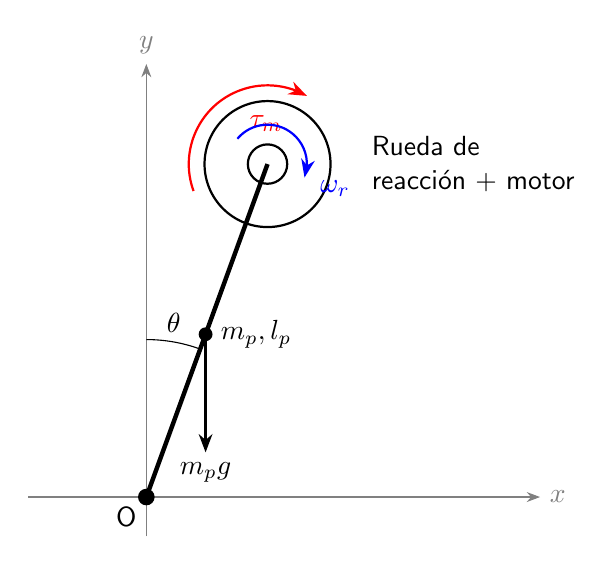
\begin{tikzpicture}[>=Stealth, font=\sffamily]
        % Ejes coordenados
        \draw[gray, ->] (-1.5,0) -- (5,0) node[right] {$x$};
        \draw[gray, ->] (0,-0.5) -- (0,5.5) node[above] {$y$};
        \node[below left] at (0,0) {O};

        % Coordenadas del brazo
        \coordinate (O) at (0,0);
        \coordinate (End) at (70:4.5); % Ángulo desde X (equivale a 20° desde Y)
        \coordinate (CMp) at (70:2.2);

        % Brazo del péndulo
        \draw[ultra thick] (O) -- (End);
        \fill (O) circle (3pt);

        % Ángulo theta
        \draw (0,2) arc (90:70:2) node[midway, above] {$\theta$};

        % Centro de masa (mp, lp)
        \fill (CMp) circle (2.5pt);
        \node[right=2pt] at (CMp) {$m_p, l_p$};
        \draw[->, thick] (CMp) -- ++(0,-1.5) node[below] {$m_pg$};

        % Rueda de reacción y motor
        \draw[thick] (End) circle (0.8);
        \draw[thick] (End) circle (0.25);
        \node[right=1.2cm, align=left] at (End) {Rueda de \\ reacción + motor};

        % Torques y velocidades (flechas curvas)
        \draw[->, red, thick] ($(End)+(200:1)$) arc (200:60:1) node[left=5pt, yshift=-10pt] {$\tau_m$};
        \draw[->, blue, thick] ($(End)+(140:0.5)$) arc (140:-20:0.5) node[right=2pt, yshift=-4pt] {$\omega_r$};
    \end{tikzpicture}%
    }
    \caption{Esquema del péndulo invertido con rueda de reacción (RWIP) de referencia de la guía.}
    \label{fig:pendulo_referencia}
\end{figure}
\subsection{Modelamiento del sistema}
Para el modelamiento del sistema presentado en la figura \ref{fig:pendulo_referencia}, se requieren realizar algunas variaciones debido a su estructura ya implementado, como se muestra en la figura \ref{fig:pendulo_implementado}
\begin{figure}[htbp]
    \centering
    \resizebox{\columnwidth}{!}{%
    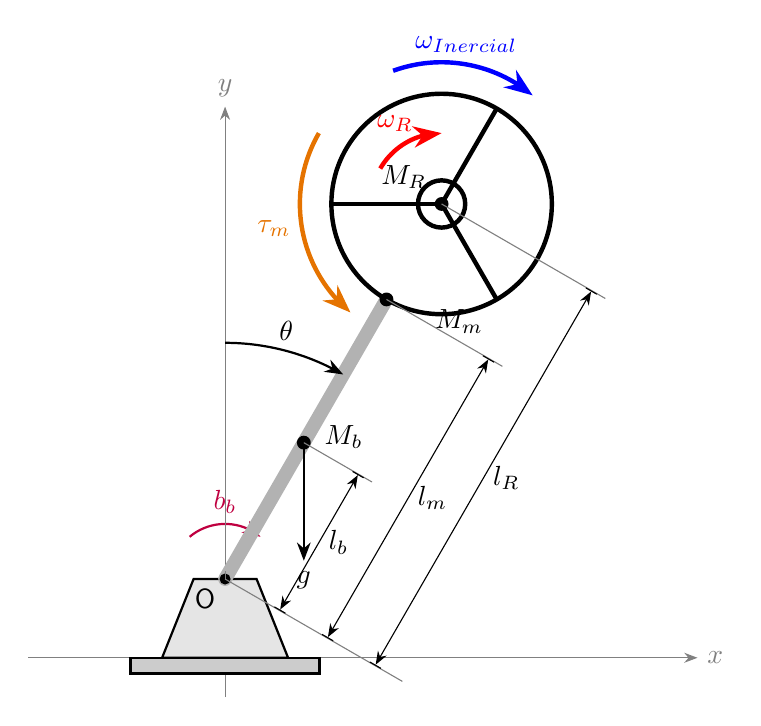
\begin{tikzpicture}[>=Stealth, font=\sffamily]
        % Ejes coordenados (y hacia arriba)
        \draw[gray, ->] (-2.5,0) -- (6,0) node[right] {$x$};
        \draw[gray, ->] (0,-0.5) -- (0,7) node[above] {$y$};
        
        % Soporte base esquemático
        \draw[thick, fill=gray!20] (-0.8,0) -- (-0.4,1) -- (0.4,1) -- (0.8,0) -- cycle;
        \draw[thick, fill=gray!40] (-1.2,-0.2) rectangle (1.2,0);
        
        % Redefinir origen en el pivote
        \coordinate (O) at (0,1);
        \node[below left] at (O) {O};
        \def\angle{30} % Ángulo theta desde el eje Y
        
        % Fricción viscosa b_b en el pivote
        \draw[->, thick, purple] ($(O)+(130:0.7)$) arc (130:50:0.7) node[midway, above] {$b_b$};
        
        % Coordenadas a lo largo del brazo (90 - 30 = 60 grados)
        \coordinate (End) at ($(O) + (60:5.5)$);
        \coordinate (CMb) at ($(O) + (60:2)$);
        \coordinate (CMm) at ($(O) + (60:4.1)$);
        \coordinate (CMr) at ($(O) + (60:5.5)$);
        
        % Brazo del péndulo
        \draw[line width=5pt, gray!60, line cap=round] (O) -- (End);
        \fill (O) circle (2pt);
        
        % Línea de referencia eje Y
        \draw[dashed, gray] (O) -- (0,6.5);
        
        % Ángulo theta (desde Y positivo hacia el brazo)
        \draw[->, thick] ($(O)+(0,3)$) arc (90:60:3) node[midway, above] {$\theta$};
        
        % ---------------------------------------------------------
        % RUEDA DE REACCIÓN
        % ---------------------------------------------------------
        \draw[ultra thick, fill=white] (CMr) circle (1.4);
        \draw[ultra thick] (CMr) circle (0.3);
        % Radios de la rueda
        \draw[ultra thick] (CMr) -- ($(CMr)+(60:1.4)$);
        \draw[ultra thick] (CMr) -- ($(CMr)+(180:1.4)$);
        \draw[ultra thick] (CMr) -- ($(CMr)+(300:1.4)$);
        \fill (CMr) circle (2.5pt); % CM Rueda
        \node[above left=2pt] at (CMr) {$M_R$}; % Etiqueta masa rueda
        
        % ---------------------------------------------------------
        % ETIQUETAS DE CENTRO DE MASA Y GRAVEDAD
        % ---------------------------------------------------------
        \fill (CMb) circle (2.5pt) node[right=4pt, yshift=2pt] {$M_b$};
        \fill (CMm) circle (2.5pt) node[right=14pt, yshift=-8pt] {$M_m$};
        
        % Vector de gravedad g iniciando en Mb
        \draw[->, thick] (CMb) -- ++(0,-1.5) node[below] {$g$};
        
        % ---------------------------------------------------------
        % LÍNEAS DE ACOTACIÓN (l_b, l_m, l_R)
        % ---------------------------------------------------------
        \draw[gray, thin] (O) -- ++(-30:2.6);
        \draw[gray, thin] (CMb) -- ++(-30:1.0);
        \draw[gray, thin] (CMm) -- ++(-30:1.7);
        \draw[gray, thin] (CMr) -- ++(-30:2.4);
        
        \draw[|<->|] ($(O)+(-30:0.8)$) -- ($(CMb)+(-30:0.8)$) node[midway, right] {$l_b$};
        \draw[|<->|] ($(O)+(-30:1.5)$) -- ($(CMm)+(-30:1.5)$) node[midway, right] {$l_m$};
        \draw[|<->|] ($(O)+(-30:2.2)$) -- ($(CMr)+(-30:2.2)$) node[midway, right] {$l_R$};
        
        % ---------------------------------------------------------
        % VELOCIDADES ANGULARES Y TORQUE
        % ---------------------------------------------------------
        % omega_Inercial (absoluta) a radio 1.8
        \draw[->, ultra thick, blue] ($(CMr)+(110:1.8)$) arc (110:50:1.8) node[midway, above] {$\omega_{Inercial}$};
        
        % omega_R (relativa al brazo) a radio 0.9 (sentido horario)
        \draw[->, ultra thick, red] ($(CMr)+(150:0.9)$) arc (150:90:0.9) node[midway, left=4pt, above] {$\omega_R$};
        
        % Torque de control tau_m (Motor) a radio 1.8 (sentido antihorario, opuesto a omega_R)
        \draw[->, ultra thick, orange!90!black] ($(CMr)+(150:1.8)$) arc (150:230:1.8) node[midway, left] {$\tau_m$};
        
    \end{tikzpicture}%
    }
    \caption{Diagrama cinemático y dinámico del péndulo invertido implementado.}
    \label{fig:pendulo_implementado}
\end{figure}
\subsubsection{Abreviaciones}
En la figura \ref{fig:pendulo_implementado} cada una de las abreviaciones corresponde a lo siguiente:
\begin{itemize}
    \item \textbf{$M_m$}: Masa del motor.
    \item \textbf{$M_R$}: Masa de la rueda de reacción.
    \item \textbf{$M_b$}: Masa del brazo del péndulo.
    \item \textbf{$b_b$}: Fricción viscosa en el eje del brazo del péndulo.
    \item \textbf{$b_m$}: Fricción viscosa del motor.
    \item \textbf{$l_b$}: Distancia del centro de masa del brazo del péndulo al eje de pivote.
    \item \textbf{$l_m$}: Distancia del centro de masa del motor al eje de pivote.
    \item \textbf{$l_R$}: Distancia del centro de masa de la rueda de reacción al eje de pivote.
    \item \textbf{$g$}: Aceleración de la gravedad.
    \item \textbf{$\tau_m$}: Torque de control efectivo del motor.
    \item \textbf{$I_{bo}$}: Inercia del péndulo con respecto al punto de origen O.
    \item \textbf{$I_{ro}$}: Inercia de la rueda de reacción con respecto al punto de origen O.
    \item \textbf{$I_{mo}$}: Inercia del motor con respecto al punto de origen O.
    \item \textbf{$I_R$}: Inercia de la rueda de reacción con respecto a su propio centro de masa.
    \item \textbf{$\omega_R$}: Velocidad angular de la rueda con respecto al brazo del péndulo.
    \item \textbf{$\omega_{Inercial}$}: Velocidad angular inercial (absoluta) de la rueda.
    \item \textbf{$\theta$}: Ángulo de inclinación del péndulo medido desde el eje vertical de referencia.
    \item \textbf{$O$}: Punto de pivote en la base y origen del sistema de coordenadas cartesianas.
\end{itemize}
Teniendo en cuenta la figura \ref{fig:pendulo_implementado}, y de acuerdo con la ecuación \eqref{eq:sumatoria_torque}, donde $I$ es el momento inercial y $\alpha$ es la aceleración angular.
\begin{equation}
    \sum \tau = I \alpha
    \label{eq:sumatoria_torque}
\end{equation}
Se plantean las ecuaciones \eqref{eq:sumatoria_torque_motor} y \eqref{eq:sumatoria_torque_base}. Que representan la sumatoria del torque del motor y del brazo respectivamente.
\begin{equation}
    \tau_m= I_{R} \cdot \dot{w}_{Inercial}
    \label{eq:sumatoria_torque_motor}
\end{equation}
\begin{equation}
   \tau_b= I_{t}\ddot{\theta}= k \sin(\theta)-b_b \dot{\theta}-\tau_m
    \label{eq:sumatoria_torque_base}
\end{equation}
Donde $w_{Incercial}$ se define como
\begin{equation}
    w_{Incercial}=\dot{\theta}+w_r
    \label{eq:w_inercial_ecuacion}
\end{equation}
Donde $b_b$ es el coeficiente de fricción que posee la rueda y k es la magnitud del torque generado por la gravedad, se define con la ecuación \eqref{eq:momento_incercial_gravedad} e $I_t$ el momento inercial total del sistema definido en la ecuación \eqref{eq:momento_incercial_total}
\begin{equation}
    k= (l_b\cdot M_b+M_m\cdot l_m+M_Rl_R)\cdot g
    \label{eq:momento_incercial_gravedad}
\end{equation}
\begin{equation}
    I_t=I_{mo}+I_{ro}+I_{bo}
    \label{eq:momento_incercial_total}
\end{equation}
La ecuación \eqref{eq:sumatoria_torque_motor}, se puede escribir teniendo en cuenta el torque eléctrico ($\tau_e$), como en la ecuación \eqref{eq:torque_motor_electrico}
\begin{equation}
 \tau_m=  \tau_e-b_m w_r 
    \label{eq:torque_motor_electrico}
\end{equation}
Donde el $\tau_e$ se define en la ecuación \eqref{eq:torque_electrico}, donde $i(t)$ es la corriente del motor en el tiempo y $k_i$ es la constante de torque del motor
\begin{equation}
    \tau_e=k_i \cdot i(t)
    \label{eq:torque_electrico}
\end{equation}

Teniendo todas las ecuaciones de la parte mecánica del sistema, faltan obtener las ecuaciones de la parte eléctrica que posee el motor donde su equivalente es la figura \ref{fig:circuito_motor}. Aplicando LK  se obtiene la siguiente ecuación
\begin{equation*}
    v(t)= \text{L}\frac{di(t)}{dt}+\text{R}\cdot i(t)+e(t)
\end{equation*}

\begin{equation}
    v(t)= \text{L}\frac{di(t)}{dt}+\text{R}\cdot i(t)+k_e w_r
    \label{eq:modelo_electrico_motor}
\end{equation}
\begin{figure}[htbp]
    \centering
    \begin{circuitikz}[american]
        % Rama inferior: Cierre del circuito
        \draw (0,0) to[short] (5.5,0);
        
        % Rama izquierda: Fuente de voltaje (american voltage source)
        % Se dibuja desde (0,3) hasta (0,0) para que el signo + quede arriba.
        % 'l_=' asegura que la etiqueta quede por fuera (a la izquierda).
        \draw (0,3) to[american voltage source, l_=$v(t)$] (0,0);
        
        % Rama superior: Corriente i(t), Inductor L_a, Resistencia R_a
        \draw (0,3) to[short, i=$i(t)$] (1.5,3)
                    to[L, l=$L_a$] (3.5,3)
                    to[R, l=$R_a$] (5.5,3);
                    
        % Rama derecha: Motor usando el nodo nativo 'elmech'
        \node[elmech] (M) at (5.5,1.5) {M};
        \draw (5.5,0) -- (M.south);
        \draw (M.north) -- (5.5,3);
        
        % Etiqueta del motor (centrada a la derecha)
        \node[right=6pt] at (M.east) {$e(t) = k_e\omega_r$};
        
    \end{circuitikz}
    \caption{Circuito eléctrico equivalente del motor de corriente continua.}
    \label{fig:circuito_motor}
\end{figure}
\subsection{Linealización del modelo}
Como la ecuación \eqref{eq:momento_incercial_gravedad} es un ecuación no lineal, se linealiza para valores $\theta$ muy pequeños, esto permite tener un rango de valores para cual  se cumple la siguiente relación
\begin{equation}
    \sin{\theta}\approx  \theta
    \label{eq:approx_sin_angulo}
\end{equation}
Esto se puede comprobar en las gráficas \ref{fig:grafica_seno_valores_lineales_grados} y \ref{fig:grafica_seno_valores_lineales_radianes}, que tiene valores lineales de la ecuación \eqref{eq:approx_sin_angulo} comparada con la $\sin \theta$ real, donde el intervalo $[-31.6, 31.6]$° o $[-0.55, 0.55]$ rad, son valores que tienen errores menores al 5\%, lo cual hace mas exacto la linealización
\begin{figure}[htbp]
\centerline{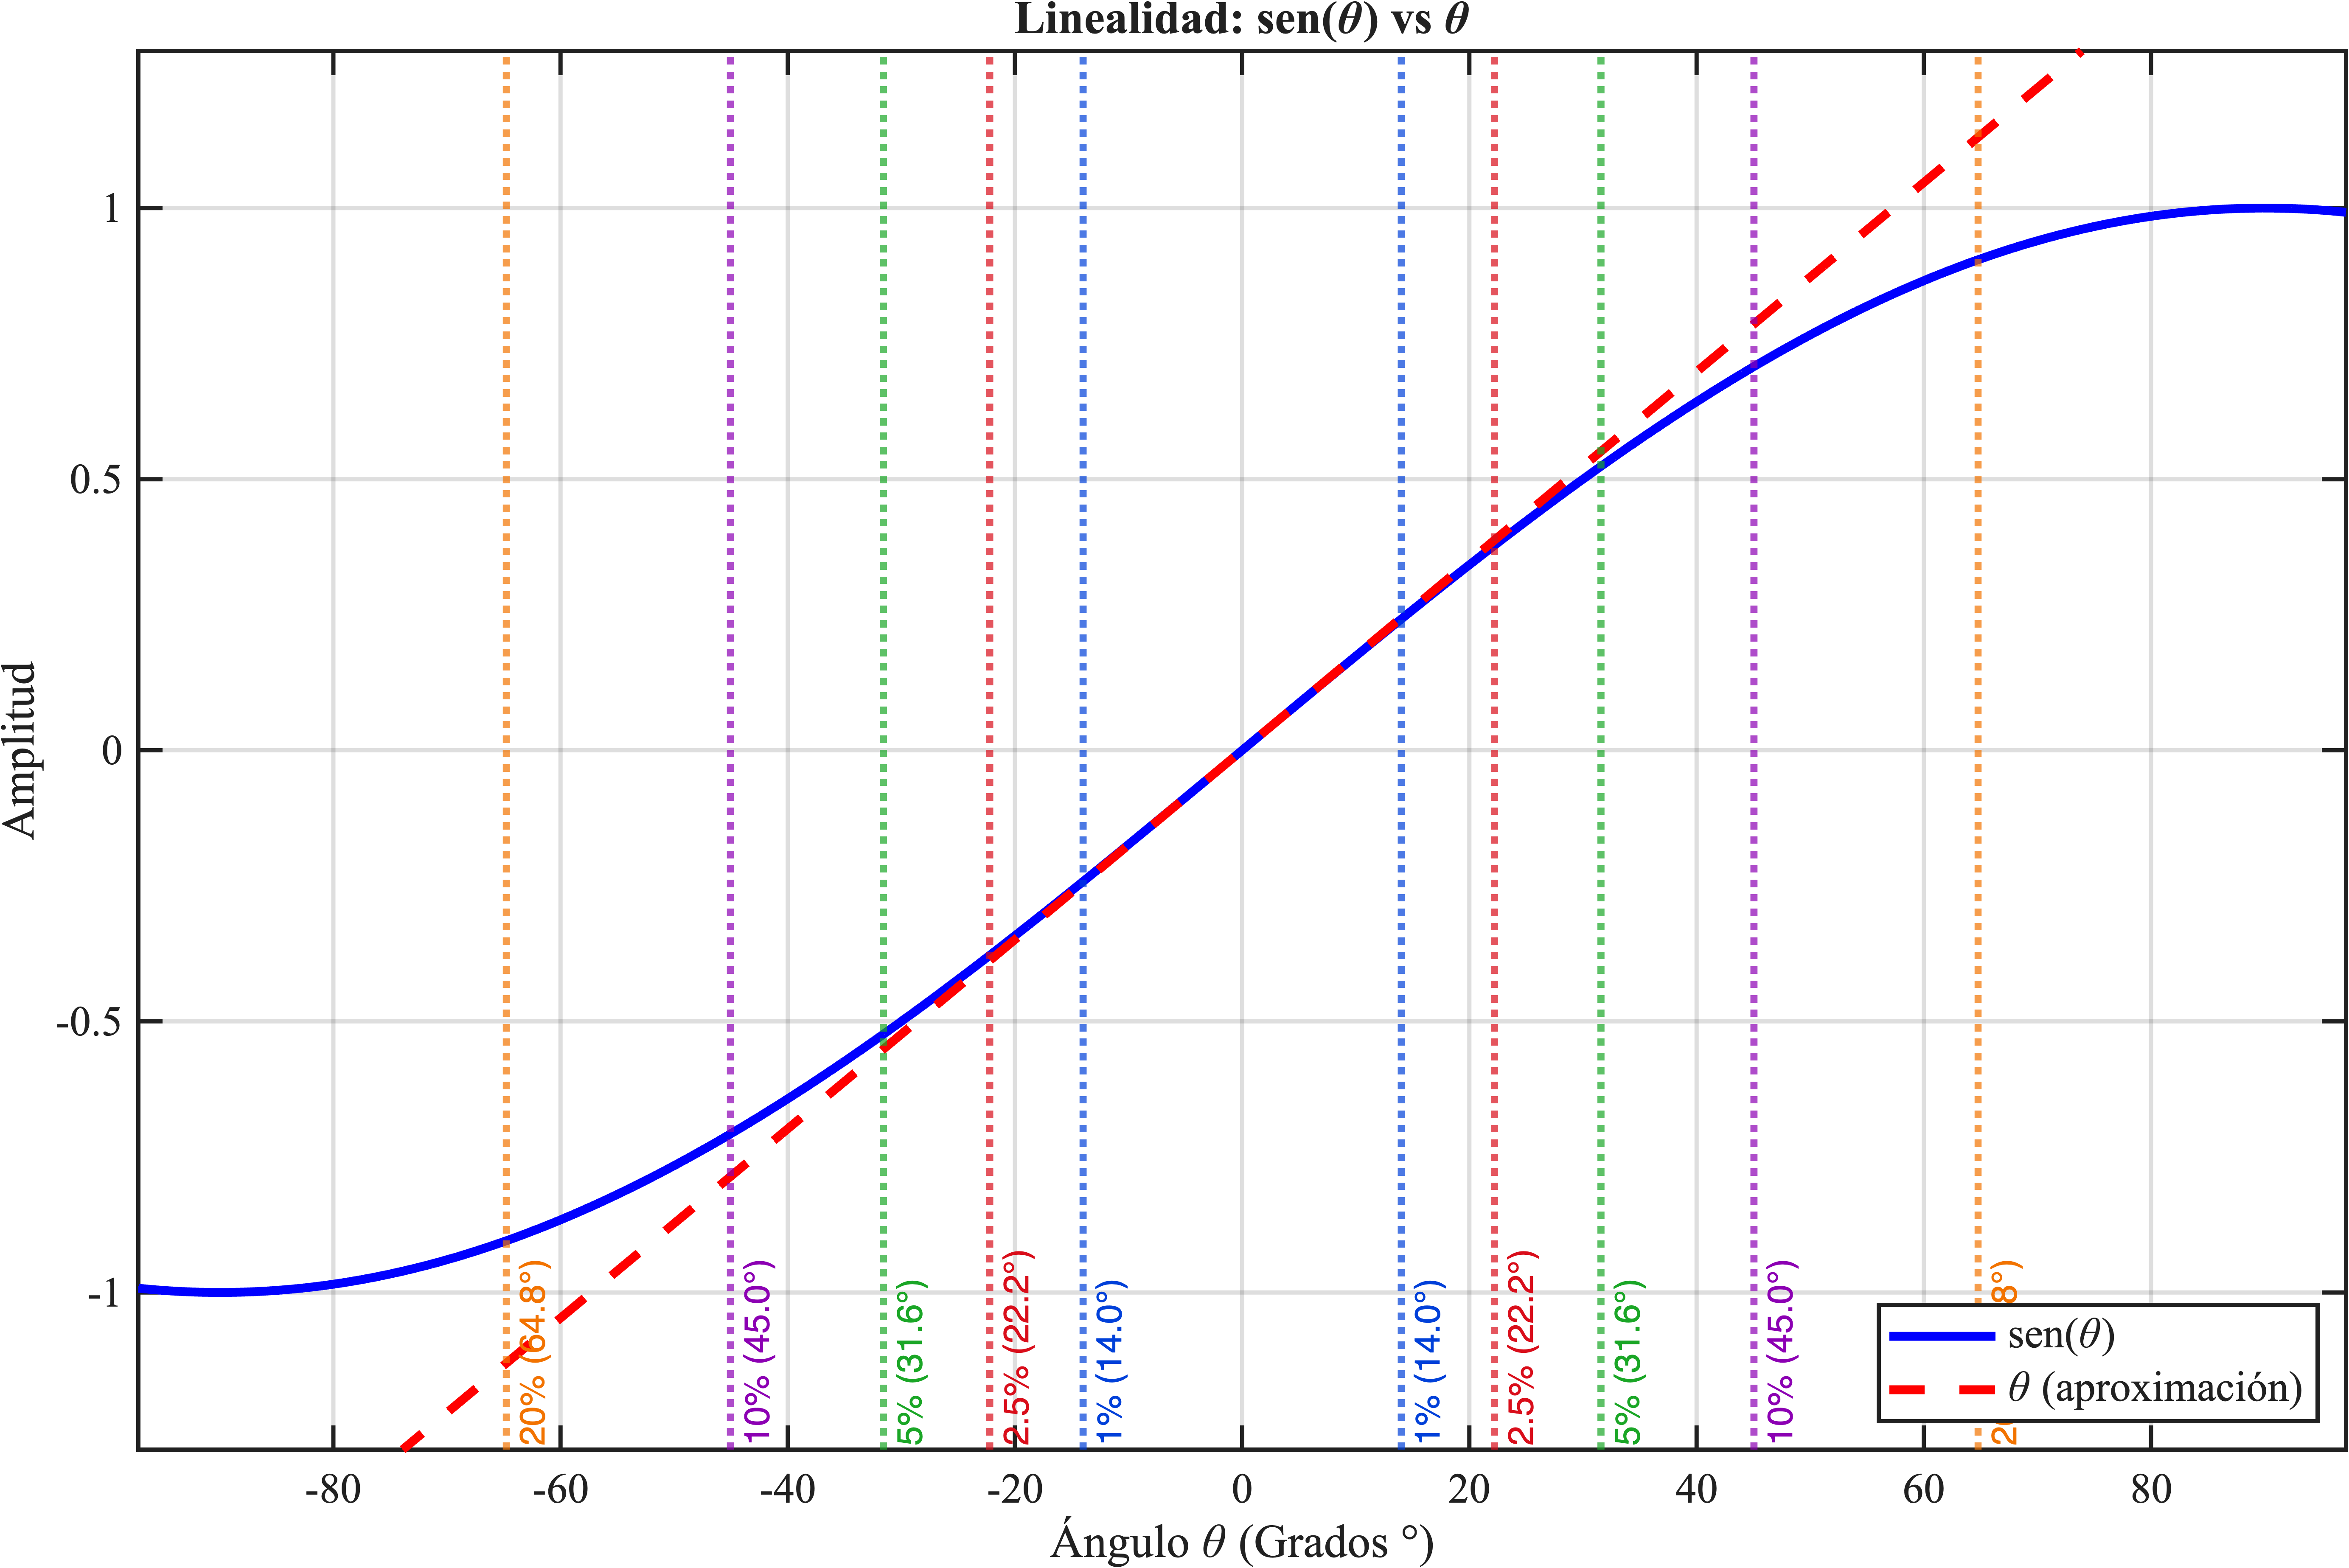
\includegraphics[width=\columnwidth]{img/linealidad_seno/Fig1_Linealidad_Grados.png}}
\caption{Valores para cual $\sin{\theta}$ es lineal grados}
\label{fig:grafica_seno_valores_lineales_grados}
\end{figure}

\begin{figure}[htbp]
\centerline{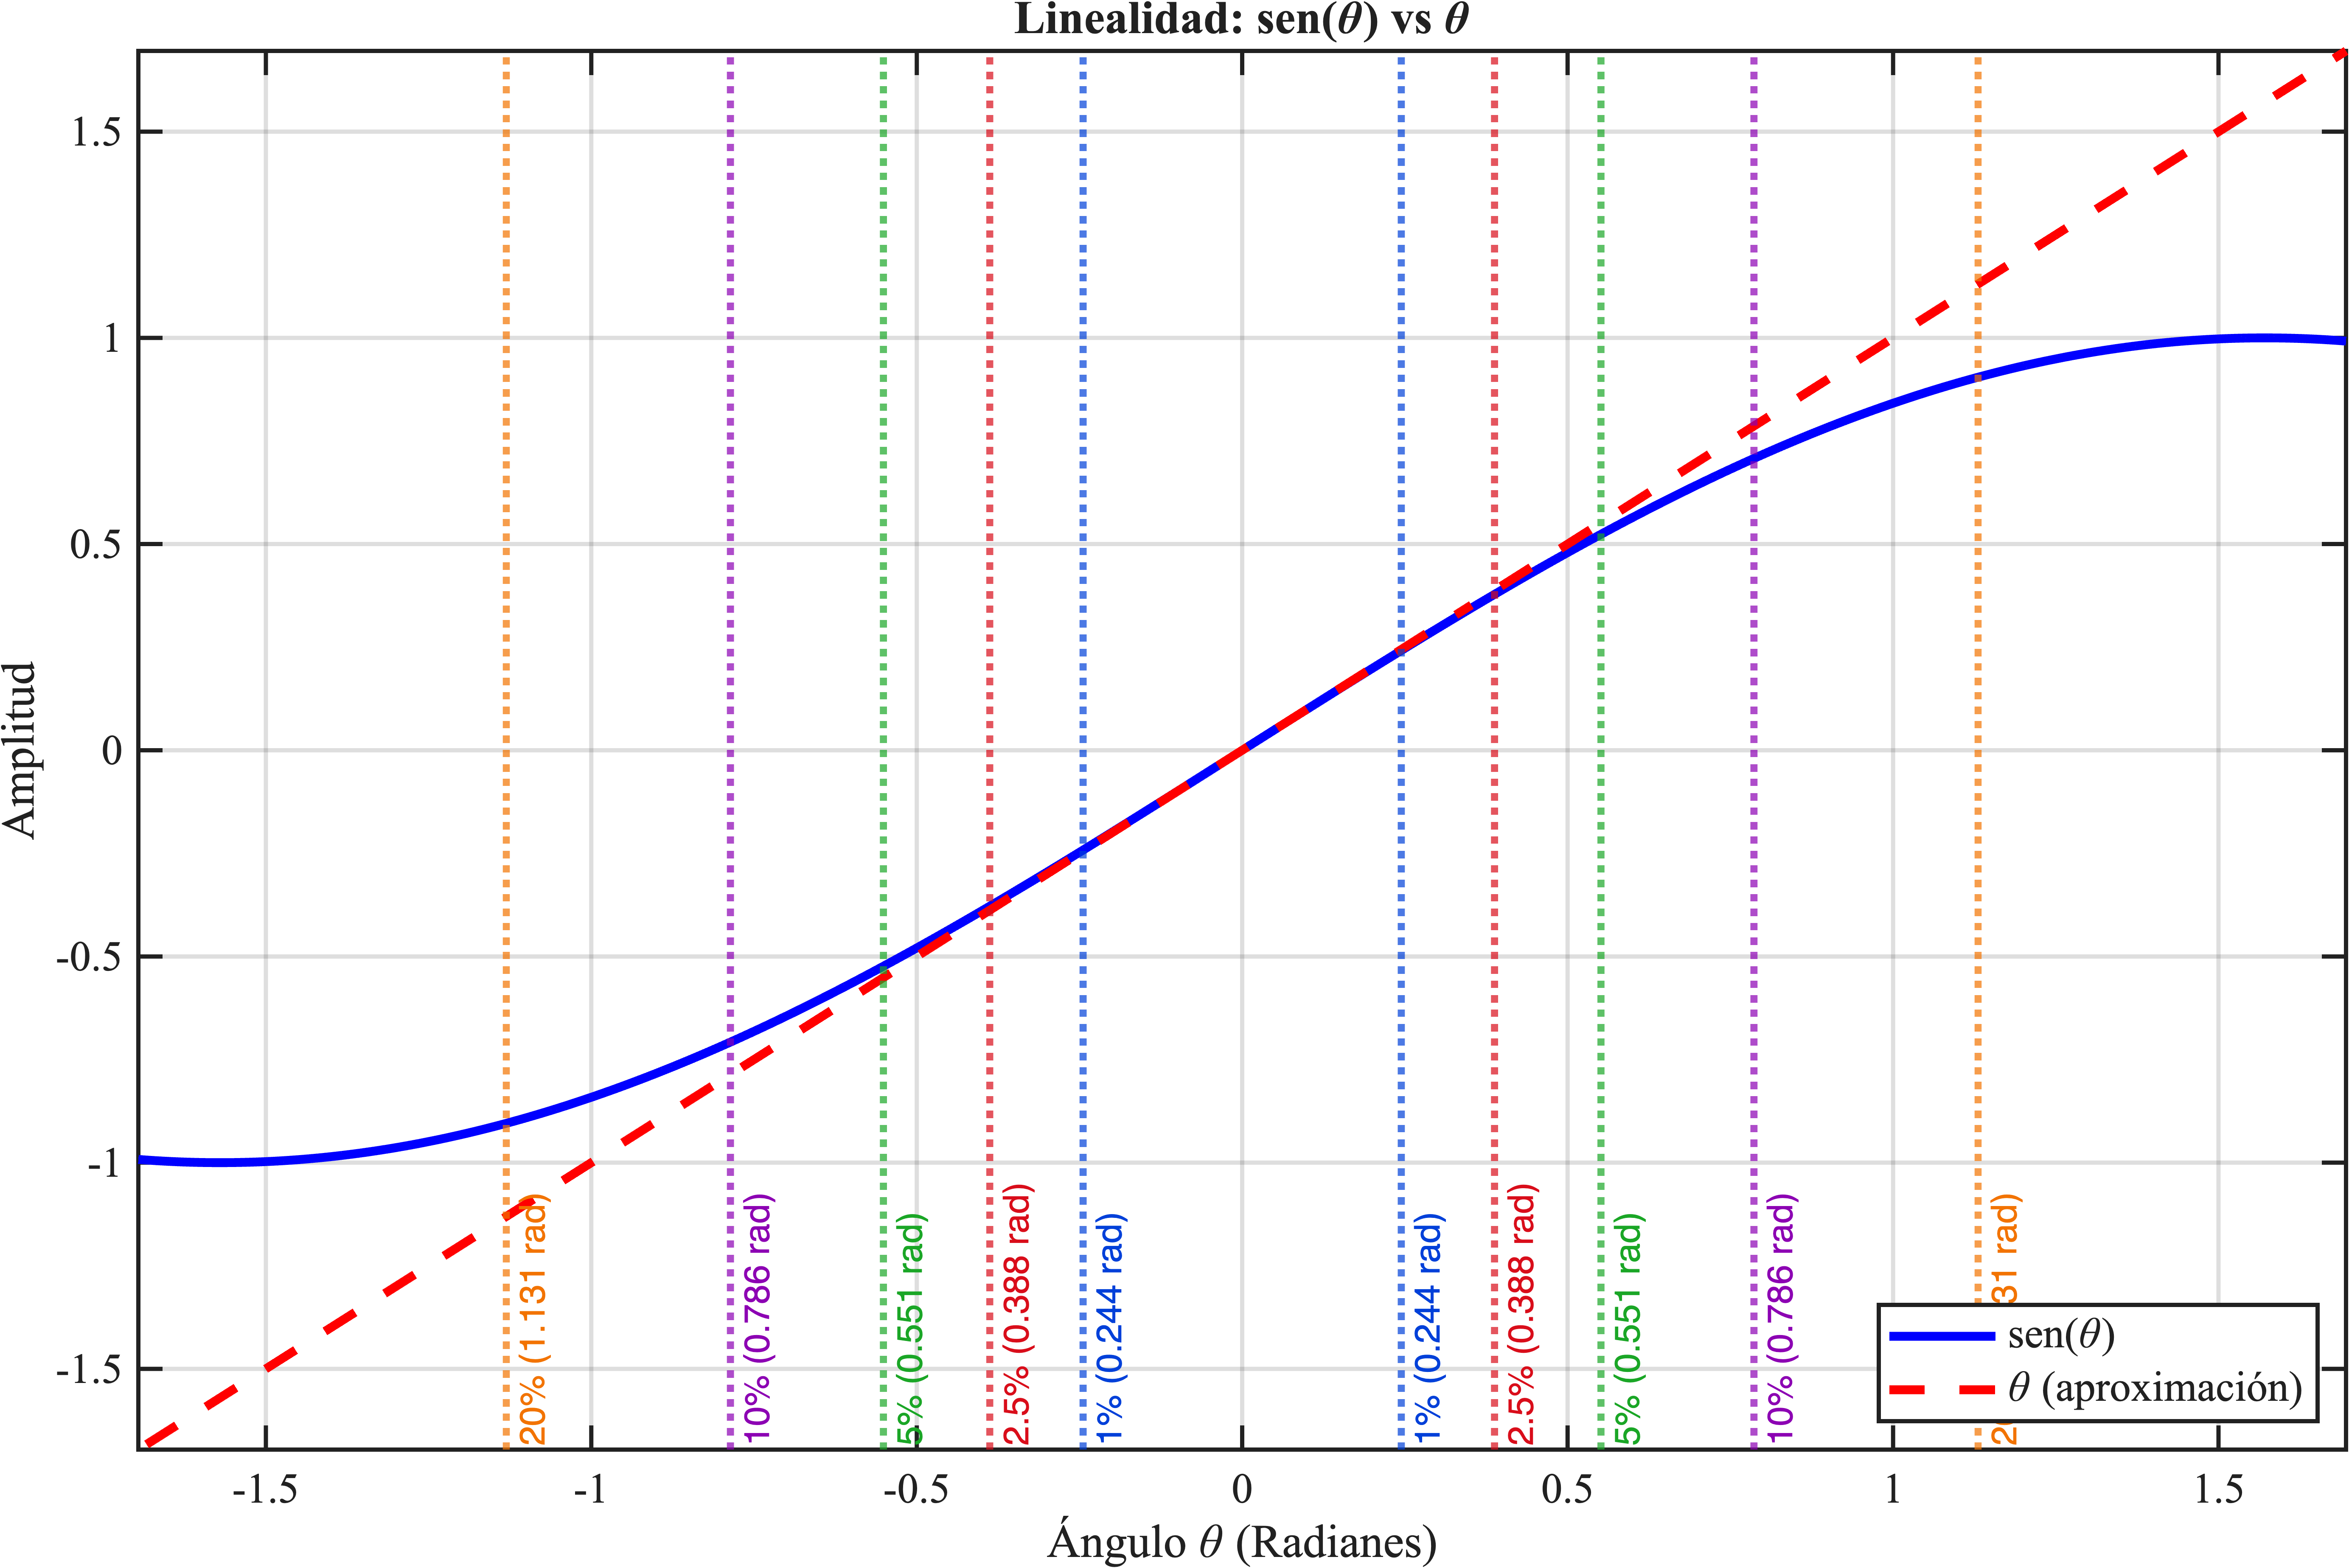
\includegraphics[width=\columnwidth]{img/linealidad_seno/Fig3_Linealidad_Radianes.png}}
\caption{Valores para cual $\sin{\theta}$ es lineal radianes}
\label{fig:grafica_seno_valores_lineales_radianes}
\end{figure}
Teniendo en cuenta la linealidad de la ecuación \eqref{eq:approx_sin_angulo}, se puede reescribir la ecuacion \eqref{eq:momento_incercial_gravedad} como
\begin{equation}
    I_{t}\ddot{\theta}= k \theta-b_b \dot{\theta}-\tau_m
    \label{eq:sumatoria_torque_base_lineal}
\end{equation}
\subsection{Variables de estado del modelo}
De las ecuaciones obtenidas en la sección de modelamiento y de la linealización del sistema, se pueden obtener las siguientes variables de estados, que corresponden a los elementos que almacenan energía
\begin{enumerate}
    \item $w_r$. Energía cinética de la rueda de reacción, velocidad angular de la rueda de reacción
    \item $\theta$. Energía cinética del sistema, posición angular del sistema.
    \item $\dot{\theta}$. Energía potencial debido a la acción gravitacional. Velocidad angular del sistema.
\end{enumerate}
Se puede tener en cuenta la $i(t)$  del motor debido al elemento inductivo que almacena energia, pero como el factor $RL\approx0$ debido a la influencia del embobinado del motor con $L\approx0$ y los valores de resistencia de armadura cerca de los miliohmios se puede despreciar esta acción  y  además de las especificaciones del proyecto. Teniendo en cuenta lo anterior, se simplifica la ecuación \eqref{eq:modelo_electrico_motor} y  se obtiene la siguiente ecuación 
\begin{equation}
    v(t)= \text{R}_a\cdot i(t)+ k_e \cdot w_r
    \label{eq:modelo_electrico_motor_simplificada}
\end{equation}
Teniendo lo anterior se obtuvo las siguientes variables de estado
\begin{equation}
\underline{x}=
\begin{bmatrix}
\theta& \dot{\theta} &w_r
\end{bmatrix}^T
\end{equation}
Donde la entrada es 
\begin{equation}
    u(t)= v(t)
\end{equation}
\subsubsection{Obtención de $\dot{x_1}$}
Se puede obtener la relación de la ecuación \eqref{eq:x1'_ecuacion}, debido a que $\dot{\theta}$ es la dervida de $\theta$ 
\begin{equation}
    \dot{x}_1 =  x_2
    \label{eq:x1'_ecuacion}
\end{equation}
\subsubsection{Obtención de $\dot{x_2}$}
De la ecuación \eqref{eq:sumatoria_torque_base_lineal}, reescribimos con variables de estado y despejamos $\dot{x_2}$ dando como resultado la ecuación \eqref{eq:x2'_en_terminos_torque_m}
\begin{equation}
    \dot{x_2}=\frac{k}{I_t}x_1-\frac{b_b}{I_t}x_2-\frac{\tau_m}{I_t}
    \label{eq:x2'_en_terminos_torque_m}
\end{equation}
Despejamos $i(t)$ de la ecuación \eqref{eq:modelo_electrico_motor_simplificada} y reemplazamos en \eqref{eq:torque_electrico} dando como resultado \eqref{eq:torque_en_terminos_estados}, esta última se reemplaza en  \eqref{eq:torque_motor_electrico} y por ultimo se reemplaza en
\eqref{eq:x2'_en_terminos_torque_m}

 \begin{equation*}
     i(t)=\frac{1}{\text{R}_a}u(t)-\frac{k_e}{\text{R}_a}x_3
 \end{equation*}

 \begin{equation*}
     \tau_e=k_i\cdot(\frac{1}{\text{R}_a}u(t)-\frac{k_e}{\text{R}_a}x_3)
 \end{equation*}

 \begin{equation*}
 \tau_m=k_i\cdot(\frac{1}{\text{R}_a}u(t)-\frac{k_e}{\text{R}_a}x_3)-b_m x_3 
\end{equation*}
\begin{equation}
 \tau_m=(-b_m-\frac{k_e k_i}{\text{R}_a}) x_3 +\frac{k_i}{\text{R}_a}u(t)
 \label{eq:torque_en_terminos_estados}
\end{equation}
\begin{equation*}
    \dot{x_2}=\frac{k}{I_t}x_1-\frac{b_b}{I_t}x_2-\frac{(-b_m-\frac{k_e k_i}{\text{R}_a}) x_3 +\frac{k_i}{\text{R}_a}u(t)}{I_t}
\end{equation*}

\begin{equation}
    \dot{x_2}=\frac{k}{I_t}x_1-\frac{b_b}{I_t}x_2+\frac{b_mR_a+k_e k_i }{I_t R_a} x_3-\frac{k_i}{\text{R}_a I_t}u(t)
    \label{eq:x2'_ecuacion}
\end{equation}
\subsubsection{Obtención de $\dot{x_3}$}
Reemplazamos las ecuaciones \eqref{eq:torque_en_terminos_estados} y \eqref{eq:w_inercial_ecuacion} en la ecuación \eqref{eq:sumatoria_torque_motor}, esta ultima se reemplaza en la ecuación \eqref{eq:x2'_ecuacion} y por último se despeja $\dot{x_3}$ dando como resultado la ecuación \eqref{eq:x'3_ecuacion}

\begin{equation*}
    (-b_m-\frac{k_e k_i}{\text{R}_a}) x_3 +\frac{k_i}{\text{R}_a}u(t)= I_{R} \cdot (\dot{x_2}+\dot{x_3})
\end{equation*}

\begin{equation*}
    \dot{x_3}=-\dot{x_2}-(b_m+\frac{k_e k_i}{\text{R}_a}) \cdot\frac{1}{I_R} x_3 +\frac{k_i}{\text{R}_a I_R}u(t)
\end{equation*}
\begin{equation*}
\begin{split}
    \dot{x}_3 &= -\left(\frac{k}{I_t}x_1 - \frac{b_b}{I_t}x_2 + \frac{b_m R_a + k_e k_i}{I_t R_a} x_3 - \frac{k_i}{R_a I_t}u(t)\right) \\
    &\quad - \left(b_m + \frac{k_e k_i}{R_a}\right) \frac{1}{I_R} x_3 + \frac{k_i}{R_a I_R}u(t)
\end{split}
\end{equation*}

\begin{equation}
\begin{split}
    \dot{x}_3 &= -\frac{k}{I_t}x_1 + \frac{b_b}{I_t}x_2 \\
    &\quad - \frac{(b_m R_a + k_e k_i)(I_t + I_R)}{R_a I_t I_R}x_3 + \frac{k_i (I_t + I_R)}{R_a I_t I_R}u(t)
\end{split}
\label{eq:x'3_ecuacion}
\end{equation}
Teniendo cada uno  de las variables de estados, se arma la matriz de estado de acuerdo a la ecuación \eqref{eq:matriz_estado}
\begin{equation}
    \begin{matrix}
       \dot{\underline{x}}(t)= A \underline{x}(t) + B u(t) \\
       \underline{y}(t)= C \underline{x}(t) + D u(t)
    \end{matrix}
    \label{eq:matriz_estado}
\end{equation}
Donde las matrices A, B, C y D corresponden a las ecuaciones \eqref{eq:matriz_A}, \eqref{eq:matriz_B}, \eqref{eq:matriz_C} y \eqref{eq:matriz_D} respectivamente.

\begin{equation}
    A=\begin{bmatrix}
        0 & 1 & 0 \\
        \frac{k}{I_t} & -\frac{b_b}{I_t} & \frac{b_mR_a+k_ek_i}{I_tR_a} \\
        -\frac{k}{I_t} & \frac{b_b}{I_t} & \frac{(b_m R_a + k_e k_i)(I_t + I_R)}{R_a I_t I_R}
    \end{bmatrix}
    \label{eq:matriz_A}
\end{equation}
\begin{equation}
    B=\begin{bmatrix}
        0 \\
        -\frac{k_i}{\text{R}_a I_t} \\
        \frac{k_i (I_t + I_R)}{R_a I_t I_R}   
    \end{bmatrix}
    \label{eq:matriz_B}   
\end{equation}
\begin{equation}
    C=\begin{bmatrix}
        1 & 0 & 0\\
        0 & 1 & 0 \\
        0 & 0 & 1
    \end{bmatrix}
    \label{eq:matriz_C}   
\end{equation}
\begin{equation}
   D = 0
    \label{eq:matriz_D}   
\end{equation}
\section{Prepare Your Paper Before Styling}
Before you begin to format your paper, first write and save the content as a 
separate text file. Complete all content and organizational editing before 
formatting. Please note sections \ref{AA}--\ref{SCM} below for more information on 
proofreading, spelling and grammar.

Keep your text and graphic files separate until after the text has been 
formatted and styled. Do not number text heads---{\LaTeX} will do that 
for you.

\subsection{Abbreviations and Acronyms}\label{AA}
Define abbreviations and acronyms the first time they are used in the text, 
even after they have been defined in the abstract. Abbreviations such as 
IEEE, SI, MKS, CGS, ac, dc, and rms do not have to be defined. Do not use 
abbreviations in the title or heads unless they are unavoidable.

\subsection{Units}
\begin{itemize}
\item Use either SI (MKS) or CGS as primary units. (SI units are encouraged.) English units may be used as secondary units (in parentheses). An exception would be the use of English units as identifiers in trade, such as ``3.5-inch disk drive''.
\item Avoid combining SI and CGS units, such as current in amperes and magnetic field in oersteds. This often leads to confusion because equations do not balance dimensionally. If you must use mixed units, clearly state the units for each quantity that you use in an equation.
\item Do not mix complete spellings and abbreviations of units: ``Wb/m\textsuperscript{2}'' or ``webers per square meter'', not ``webers/m\textsuperscript{2}''. Spell out units when they appear in text: ``. . . a few henries'', not ``. . . a few H''.
\item Use a zero before decimal points: ``0.25'', not ``.25''. Use ``cm\textsuperscript{3}'', not ``cc''.)
\end{itemize}

\subsection{Equations}
Number equations consecutively. To make your 
equations more compact, you may use the solidus (~/~), the exp function, or 
appropriate exponents. Italicize Roman symbols for quantities and variables, 
but not Greek symbols. Use a long dash rather than a hyphen for a minus 
sign. Punctuate equations with commas or periods when they are part of a 
sentence, as in:
\begin{equation}
a+b=\gamma\label{eq}
\end{equation}

Be sure that the 
symbols in your equation have been defined before or immediately following 
the equation. Use ``\eqref{eq}'', not ``Eq.~\eqref{eq}'' or ``equation \eqref{eq}'', except at 
the beginning of a sentence: ``Equation \eqref{eq} is . . .''

\subsection{\LaTeX-Specific Advice}

Please use ``soft'' (e.g., \verb|\eqref{Eq}|) cross references instead
of ``hard'' references (e.g., \verb|(1)|). That will make it possible
to combine sections, add equations, or change the order of figures or
citations without having to go through the file line by line.

Please don't use the \verb|{eqnarray}| equation environment. Use
\verb|{align}| or \verb|{IEEEeqnarray}| instead. The \verb|{eqnarray}|
environment leaves unsightly spaces around relation symbols.

Please note that the \verb|{subequations}| environment in {\LaTeX}
will increment the main equation counter even when there are no
equation numbers displayed. If you forget that, you might write an
article in which the equation numbers skip from (17) to (20), causing
the copy editors to wonder if you've discovered a new method of
counting.

{\BibTeX} does not work by magic. It doesn't get the bibliographic
data from thin air but from .bib files. If you use {\BibTeX} to produce a
bibliography you must send the .bib files. 

{\LaTeX} can't read your mind. If you assign the same label to a
subsubsection and a table, you might find that Table I has been cross
referenced as Table IV-B3. 

{\LaTeX} does not have precognitive abilities. If you put a
\verb|\label| command before the command that updates the counter it's
supposed to be using, the label will pick up the last counter to be
cross referenced instead. In particular, a \verb|\label| command
should not go before the caption of a figure or a table.

Do not use \verb|\nonumber| inside the \verb|{array}| environment. It
will not stop equation numbers inside \verb|{array}| (there won't be
any anyway) and it might stop a wanted equation number in the
surrounding equation.

\subsection{Some Common Mistakes}\label{SCM}
\begin{itemize}
\item The word ``data'' is plural, not singular.
\item The subscript for the permeability of vacuum $\mu_{0}$, and other common scientific constants, is zero with subscript formatting, not a lowercase letter ``o''.
\item In American English, commas, semicolons, periods, question and exclamation marks are located within quotation marks only when a complete thought or name is cited, such as a title or full quotation. When quotation marks are used, instead of a bold or italic typeface, to highlight a word or phrase, punctuation should appear outside of the quotation marks. A parenthetical phrase or statement at the end of a sentence is punctuated outside of the closing parenthesis (like this). (A parenthetical sentence is punctuated within the parentheses.)
\item A graph within a graph is an ``inset'', not an ``insert''. The word alternatively is preferred to the word ``alternately'' (unless you really mean something that alternates).
\item Do not use the word ``essentially'' to mean ``approximately'' or ``effectively''.
\item In your paper title, if the words ``that uses'' can accurately replace the word ``using'', capitalize the ``u''; if not, keep using lower-cased.
\item Be aware of the different meanings of the homophones ``affect'' and ``effect'', ``complement'' and ``compliment'', ``discreet'' and ``discrete'', ``principal'' and ``principle''.
\item Do not confuse ``imply'' and ``infer''.
\item The prefix ``non'' is not a word; it should be joined to the word it modifies, usually without a hyphen.
\item There is no period after the ``et'' in the Latin abbreviation ``et al.''.
\item The abbreviation ``i.e.'' means ``that is'', and the abbreviation ``e.g.'' means ``for example''.
\end{itemize}
An excellent style manual for science writers is \cite{b7}.

\subsection{Authors and Affiliations}
\textbf{The class file is designed for, but not limited to, six authors.} A 
minimum of one author is required for all conference articles. Author names 
should be listed starting from left to right and then moving down to the 
next line. This is the author sequence that will be used in future citations 
and by indexing services. Names should not be listed in columns nor group by 
affiliation. Please keep your affiliations as succinct as possible (for 
example, do not differentiate among departments of the same organization).

\subsection{Identify the Headings}
Headings, or heads, are organizational devices that guide the reader through 
your paper. There are two types: component heads and text heads.

Component heads identify the different components of your paper and are not 
topically subordinate to each other. Examples include Acknowledgments and 
References and, for these, the correct style to use is ``Heading 5''. Use 
``figure caption'' for your Figure captions, and ``table head'' for your 
table title. Run-in heads, such as ``Abstract'', will require you to apply a 
style (in this case, italic) in addition to the style provided by the drop 
down menu to differentiate the head from the text.

Text heads organize the topics on a relational, hierarchical basis. For 
example, the paper title is the primary text head because all subsequent 
material relates and elaborates on this one topic. If there are two or more 
sub-topics, the next level head (uppercase Roman numerals) should be used 
and, conversely, if there are not at least two sub-topics, then no subheads 
should be introduced.

\subsection{Figures and Tables}
\paragraph{Positioning Figures and Tables} Place figures and tables at the top and 
bottom of columns. Avoid placing them in the middle of columns. Large 
figures and tables may span across both columns. Figure captions should be 
below the figures; table heads should appear above the tables. Insert 
figures and tables after they are cited in the text. Use the abbreviation 
``Fig.~\ref{fig}'', even at the beginning of a sentence.

\begin{table}[htbp]
\caption{Table Type Styles}
\begin{center}
\begin{tabular}{|c|c|c|c|}
\hline
\textbf{Table}&\multicolumn{3}{|c|}{\textbf{Table Column Head}} \\
\cline{2-4} 
\textbf{Head} & \textbf{\textit{Table column subhead}}& \textbf{\textit{Subhead}}& \textbf{\textit{Subhead}} \\
\hline
copy& More table copy$^{\mathrm{a}}$& &  \\
\hline
\multicolumn{4}{l}{$^{\mathrm{a}}$Sample of a Table footnote.}
\end{tabular}
\label{tab1}
\end{center}
\end{table}

\begin{figure}[htbp]
\centerline{\includegraphics{fig1.png}}
\caption{Example of a figure caption.}
\label{fig}
\end{figure}

Figure Labels: Use 8 point Times New Roman for Figure labels. Use words 
rather than symbols or abbreviations when writing Figure axis labels to 
avoid confusing the reader. As an example, write the quantity 
``Magnetization'', or ``Magnetization, M'', not just ``M''. If including 
units in the label, present them within parentheses. Do not label axes only 
with units. In the example, write ``Magnetization (A/m)'' or ``Magnetization 
\{A[m(1)]\}'', not just ``A/m''. Do not label axes with a ratio of 
quantities and units. For example, write ``Temperature (K)'', not 
``Temperature/K''.

\section*{Acknowledgment}

The preferred spelling of the word ``acknowledgment'' in America is without 
an ``e'' after the ``g''. Avoid the stilted expression ``one of us (R. B. 
G.) thanks $\ldots$''. Instead, try ``R. B. G. thanks$\ldots$''. Put sponsor 
acknowledgments in the unnumbered footnote on the first page.

\section*{References}

Please number citations consecutively within brackets \cite{b1}. The 
sentence punctuation follows the bracket \cite{b2}. Refer simply to the reference 
number, as in \cite{b3}---do not use ``Ref. \cite{b3}'' or ``reference \cite{b3}'' except at 
the beginning of a sentence: ``Reference \cite{b3} was the first $\ldots$''

Number footnotes separately in superscripts. Place the actual footnote at 
the bottom of the column in which it was cited. Do not put footnotes in the 
abstract or reference list. Use letters for table footnotes.

Unless there are six authors or more give all authors' names; do not use 
``et al.''. Papers that have not been published, even if they have been 
submitted for publication, should be cited as ``unpublished'' \cite{b4}. Papers 
that have been accepted for publication should be cited as ``in press'' \cite{b5}. 
Capitalize only the first word in a paper title, except for proper nouns and 
element symbols.

For papers published in translation journals, please give the English 
citation first, followed by the original foreign-language citation \cite{b6}.

\begin{thebibliography}{00}

\bibitem{ref1} J. Michalski, M. Mrotek, T. Tomczak, J. Wojciechowski, and D. Pazderski, ``Reaction Wheel Pendulum Stabilization Using Various State-Space Representations,'' \textit{Electronics}, vol. 14, no. 23, p. 4719, 2025.

\bibitem{ref2} D. Zaborniak, K. Patan, and M. Witczak, ``Design, Implementation, and Control of a Wheel-Based Inverted Pendulum,'' \textit{Electronics}, vol. 13, no. 3, p. 514, 2024.

\bibitem{ref3} R. M. D. Silva, J. M. De Souza Ribeiro, R. Cardim, and M. C. Minhoto Teixeira, ``Classical and Sliding Mode Controllers Applied to the Reaction Wheel Inverted Pendulum,'' \textit{IEEE Access}, vol. 14, pp. 28884--28897, 2026.

\bibitem{ref4} Carrera de Mecatrónica UTC, ``Reaction wheel inverted pendulum,'' GitHub. \url{https://github.com/mecatronica-UTC/Reaction_wheeel_inverted_pendulum} (accedido en Octubre 2026).

\bibitem{ref5} G. Belascuen and N. Aguilar, ``Design, Modeling and Control of a Reaction Wheel Balanced Inverted Pendulum,'' in \textit{2018 IEEE Biennial Congress of Argentina (ARGENCON)}, Jun. 2018, pp. 1--9.

\bibitem{ref6} M. Gajamohan, M. Merz, I. Thommen, and R. D'Andrea, ``The Cubli: A cube that can jump up and balance,'' in \textit{2012 IEEE/RSJ International Conference on Intelligent Robots and Systems}, Vilamoura-Algarve, Portugal, 2012, pp. 3722--3727.

\end{thebibliography}
\vspace{12pt}
\color{red}
IEEE conference templates contain guidance text for composing and formatting conference papers. Please ensure that all template text is removed from your conference paper prior to submission to the conference. Failure to remove the template text from your paper may result in your paper not being published.

\end{document}
